All the testing was run on a computer using Arch Linux x86\textunderscore64, with 
a dual core processor clocked @ 2.7 GHz, and 8 GB of RAM.
I used 3 different sizes of data sets, and used different sizes of population, 
but kept the chance of mutation constant at \( \frac{1}{1000} \).
I used the number of generations to generate a correct solution to measure the
speed of the program with the different inputs.
Table~\ref*{table:results-mean} shows the mean number of generations for each
number of modules, for each population size.
The full results are in table~\ref*{table:results-full}.

\begin{table}[ht]
	\centering
	\begin{tabular}{c|ccc}
		\toprule
		& \multicolumn{3}{c}{Number of Modules} \\
		Population Size & 10 & 50 & 100 \\
		\midrule
		10 & 155 & 605 & 1205 \\
		50 & 17 & 111 & 216 \\
		100 & 11 & 73 & 162 \\
		200 & 9 & 57 & 110 \\
		\bottomrule
	\end{tabular}
	\caption{Mean average of number of generations for each number of modules
		and population size}
	\label{table:results-mean}
\end{table}

\begin{table}[ht]
	\begin{tabular}{cc|cccc|cccc|cccc}
		\toprule
		\multicolumn{2}{c}{Modules}
			& \multicolumn{4}{c}{10}
			& \multicolumn{4}{c}{50}
			& \multicolumn{4}{c}{100} \\
		\midrule
		\multicolumn{2}{c}{Population}
			& 10 & 50 & 100 & 200 
			& 10 & 50 & 100 & 200 
			& 10 & 50 & 100 & 200 \\
		\midrule
		Result & 1
			& 68 & 14 & 9 & 7
			& 391 & 103 & 80 & 55
			& 584 & 239 & 161 & 110 \\
		& 2
			& 86 & 17 & 9 & 9
			& 445 & 85 & 67 & 60
			& 777 & 204 & 145 & 115 \\
		& 3
			& 91 & 7 & 12 & 8
			& 535 & 92 & 71 & 61
			& 671 & 231 & 139 & 104 \\
		& 4
			& 117 & 10 & 11 & 8
			& 1082 & 112 & 75 & 49
			& 682 & 226 & 211 & 101 \\
		& 5
			& 265 & 9 & 10 & 10
			& 421 & 122 & 79 & 62
			& 4572 & 209 & 154 & 109 \\
		& 6
			& 157 & 24 & 13 & 12
			& 552 & 108 & 68 & 49
			& 864 & 200 & 148 & 107 \\
		& 7
			& 172 & 32 & 17 & 10
			& 580 & 126 & 66 & 55
			& 1258 & 228 & 153 & 96 \\
		& 8
			& 186 & 14 & 8 & 7
			& 802 & 120 & 71 & 54
			& 895 & 202 & 167 & 129 \\
		& 9
			& 188 & 177 & 10 & 9
			& 498 & 141 & 76 & 62
			& 928 & 191 & 177 & 101 \\
		& 10
			& 224 & 23 & 11 & 8
			& 746 & 100 & 73 & 59
			& 819 & 232 & 169 & 125 \\
		\midrule
		\multicolumn{2}{c}{Mean}
			& 155 & 17 & 11 & 9
			& 605 & 111 & 73 & 57
			& 1205 & 216 & 162 & 110 \\
		\multicolumn{2}{c}{Std Dev}
			& 64.2 & 7.7 & 2.6 & 1.6
			& 214 & 16.9 & 4.9 & 5.0
			& 1197 & 16.8 & 20.7 & 10.6 \\
		\bottomrule
	\end{tabular}
	\caption{Full testing results}
	\label{table:results-full}
\end{table}

As would be expected, increasing the size of the population reduces the number
of generations needed to produce a valid timetable.
However, there are diminishing returns with increasing the population size, as
illustrated in the graph~\ref*{fig:graph-1}.

\begin{figure}[ht]
	\centering
	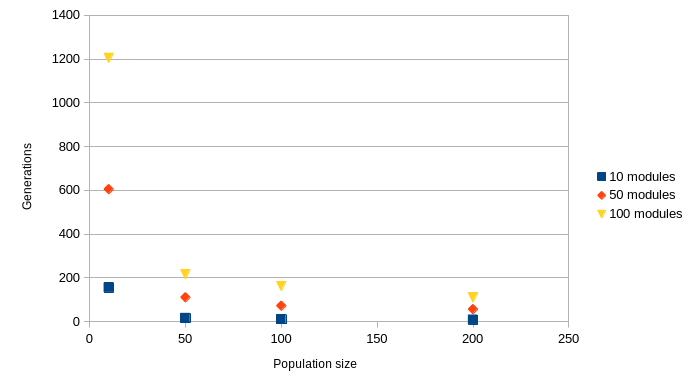
\includegraphics[scale=0.6]{images/graph-1.png}
	\caption{Graph showing generations against population size for different 
		numbers of modules}
	\label{fig:graph-1}
\end{figure}

Examples of the generated timetables are in Appendix A.